\documentclass[crop,tikz,border=2px]{standalone}
\usepackage{tikzsymbols}
\usetikzlibrary{arrows,positioning,patterns}
\begin{document}
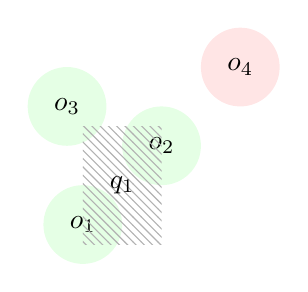
\begin{tikzpicture}[
  ur/.style={circle,minimum width=1cm,node distance=.5cm},
  cand/.style={fill=green!10},
  noncand/.style={fill=red!10},
  qry/.style={rectangle,minimum width=1cm,minimum height=1.5cm,pattern=north west lines, pattern color=black!30}]

  \node[ur,cand] (r1) at (1,1) {\(o_1\)};
  \node[ur,cand] (r2) at (2,2) {\(o_2\)};
  \node[ur,cand] (r3) at (0.8,2.5) {\(o_3\)};
  \node[ur,noncand] (r4) at (3,3) {\(o_4\)};

  \node[qry] (q) at (1.5,1.5) {\(q_1\)};
\end{tikzpicture}
\end{document}